\documentclass[conference]{IEEEtran}
\IEEEoverridecommandlockouts
% The preceding line is only needed to identify funding in the first footnote. If that is unneeded, please comment it out.
%Template version as of 6/27/2024

\usepackage{cite}
\usepackage{amsmath,amssymb,amsfonts}
\usepackage{algorithmic}
\usepackage{graphicx}
\usepackage{textcomp}
\usepackage{xcolor}
\def\BibTeX{{\rm B\kern-.05em{\sc i\kern-.025em b}\kern-.08em
    T\kern-.1667em\lower.7ex\hbox{E}\kern-.125emX}}
\begin{document}

\title{Conference Paper Title*\\
{\footnotesize \textsuperscript{*}Note: Sub-titles are not captured for https://ieeexplore.ieee.org  and
should not be used}
\thanks{Identify applicable funding agency here. If none, delete this.}
}

\author{\IEEEauthorblockN{1\textsuperscript{st} Given Name Surname}
\IEEEauthorblockA{\textit{dept. name of organization (of Aff.)} \\
\textit{name of organization (of Aff.)}\\
City, Country \\
email address or ORCID}
\and
\IEEEauthorblockN{2\textsuperscript{nd} Given Name Surname}
\IEEEauthorblockA{\textit{dept. name of organization (of Aff.)} \\
\textit{name of organization (of Aff.)}\\
City, Country \\
email address or ORCID}
\and
\IEEEauthorblockN{3\textsuperscript{rd} Given Name Surname}
\IEEEauthorblockA{\textit{dept. name of organization (of Aff.)} \\
\textit{name of organization (of Aff.)}\\
City, Country \\
email address or ORCID}
\and
\IEEEauthorblockN{4\textsuperscript{th} Given Name Surname}
\IEEEauthorblockA{\textit{dept. name of organization (of Aff.)} \\
\textit{name of organization (of Aff.)}\\
City, Country \\
email address or ORCID}
\and
\IEEEauthorblockN{5\textsuperscript{th} Given Name Surname}
\IEEEauthorblockA{\textit{dept. name of organization (of Aff.)} \\
\textit{name of organization (of Aff.)}\\
City, Country \\
email address or ORCID}
\and
\IEEEauthorblockN{6\textsuperscript{th} Given Name Surname}
\IEEEauthorblockA{\textit{dept. name of organization (of Aff.)} \\
\textit{name of organization (of Aff.)}\\
City, Country \\
email address or ORCID}
}

\maketitle

\begin{abstract}
This document is a model and instructions for \LaTeX.
This and the IEEEtran.cls file define the components of your paper [title, text, heads, etc.]. *CRITICAL: Do Not Use Symbols, Special Characters, Footnotes, 
or Math in Paper Title or Abstract.
\end{abstract}

\begin{IEEEkeywords}
component, formatting, style, styling, insert.
\end{IEEEkeywords}
\section{Introduction}
This document is a model and instructions for \LaTeX.
Please observe the conference page limits. For more information about how to become an IEEE Conference author or how to write your paper, please visit   IEEE Conference Author Center website: https://conferences.ieeeauthorcenter.ieee.org/.

\subsection{Maintaining the Integrity of the Specifications}

The IEEEtran class file is used to format your paper and style the text. All margins, 
column widths, line spaces, and text fonts are prescribed; please do not 
alter them. You may note peculiarities. For example, the head margin
measures proportionately more than is customary. This measurement 
and others are deliberate, using specifications that anticipate your paper 
as one part of the entire proceedings, and not as an independent document. 
Please do not revise any of the current designations.







\section{Prepare Your Paper Before Styling}
Before you begin to format your paper, first write and save the content as a 
separate text file. Complete all content and organizational editing before 
formatting. Please note sections \ref{AA} to \ref{FAT} below for more information on 
proofreading, spelling and grammar.

Keep your text and graphic files separate until after the text has been 
formatted and styled. Do not number text heads---{\LaTeX} will do that 
for you.

\subsection{Abbreviations and Acronyms}\label{AA}
Define abbreviations and acronyms the first time they are used in the text, 
even after they have been defined in the abstract. Abbreviations such as 
IEEE, SI, MKS, CGS, ac, dc, and rms do not have to be defined. Do not use 
abbreviations in the title or heads unless they are unavoidable.

\subsection{Units}
\begin{itemize}
\item Use either SI (MKS) or CGS as primary units. (SI units are encouraged.) English units may be used as secondary units (in parentheses). An exception would be the use of English units as identifiers in trade, such as ``3.5-inch disk drive''.
\item Avoid combining SI and CGS units, such as current in amperes and magnetic field in oersteds. This often leads to confusion because equations do not balance dimensionally. If you must use mixed units, clearly state the units for each quantity that you use in an equation.
\item Do not mix complete spellings and abbreviations of units: ``Wb/m\textsuperscript{2}'' or ``webers per square meter'', not ``webers/m\textsuperscript{2}''. Spell out units when they appear in text: ``. . . a few henries'', not ``. . . a few H''.
\item Use a zero before decimal points: ``0.25'', not ``.25''. Use ``cm\textsuperscript{3}'', not ``cc''.)
\end{itemize}

\subsection{Equations}
Number equations consecutively. To make your 
equations more compact, you may use the solidus (~/~), the exp function, or 
appropriate exponents. Italicize Roman symbols for quantities and variables, 
but not Greek symbols. Use a long dash rather than a hyphen for a minus 
sign. Punctuate equations with commas or periods when they are part of a 
sentence, as in:
\begin{equation}
a+b=\gamma\label{eq}
\end{equation}

Be sure that the 
symbols in your equation have been defined before or immediately following 
the equation. Use ``\eqref{eq}'', not ``Eq.~\eqref{eq}'' or ``equation \eqref{eq}'', except at 
the beginning of a sentence: ``Equation \eqref{eq} is . . .''

\subsection{\LaTeX-Specific Advice}

Please use ``soft'' (e.g., \verb|\eqref{Eq}|) cross references instead
of ``hard'' references (e.g., \verb|(1)|). That will make it possible
to combine sections, add equations, or change the order of figures or
citations without having to go through the file line by line.

Please don't use the \verb|{eqnarray}| equation environment. Use
\verb|{align}| or \verb|{IEEEeqnarray}| instead. The \verb|{eqnarray}|
environment leaves unsightly spaces around relation symbols.

Please note that the \verb|{subequations}| environment in {\LaTeX}
will increment the main equation counter even when there are no
equation numbers displayed. If you forget that, you might write an
article in which the equation numbers skip from (17) to (20), causing
the copy editors to wonder if you've discovered a new method of
counting.

{\BibTeX} does not work by magic. It doesn't get the bibliographic
data from thin air but from .bib files. If you use {\BibTeX} to produce a
bibliography you must send the .bib files. 

{\LaTeX} can't read your mind. If you assign the same label to a
subsubsection and a table, you might find that Table I has been cross
referenced as Table IV-B3. 

{\LaTeX} does not have precognitive abilities. If you put a
\verb|\label| command before the command that updates the counter it's
supposed to be using, the label will pick up the last counter to be
cross referenced instead. In particular, a \verb|\label| command
should not go before the caption of a figure or a table.

Do not use \verb|\nonumber| inside the \verb|{array}| environment. It
will not stop equation numbers inside \verb|{array}| (there won't be
any anyway) and it might stop a wanted equation number in the
surrounding equation.

\subsection{Some Common Mistakes}\label{SCM}
\begin{itemize}
\item The word ``data'' is plural, not singular.
\item The subscript for the permeability of vacuum $\mu_{0}$, and other common scientific constants, is zero with subscript formatting, not a lowercase letter ``o''.
\item In American English, commas, semicolons, periods, question and exclamation marks are located within quotation marks only when a complete thought or name is cited, such as a title or full quotation. When quotation marks are used, instead of a bold or italic typeface, to highlight a word or phrase, punctuation should appear outside of the quotation marks. A parenthetical phrase or statement at the end of a sentence is punctuated outside of the closing parenthesis (like this). (A parenthetical sentence is punctuated within the parentheses.)
\item A graph within a graph is an ``inset'', not an ``insert''. The word alternatively is preferred to the word ``alternately'' (unless you really mean something that alternates).
\item Do not use the word ``essentially'' to mean ``approximately'' or ``effectively''.
\item In your paper title, if the words ``that uses'' can accurately replace the word ``using'', capitalize the ``u''; if not, keep using lower-cased.
\item Be aware of the different meanings of the homophones ``affect'' and ``effect'', ``complement'' and ``compliment'', ``discreet'' and ``discrete'', ``principal'' and ``principle''.
\item Do not confuse ``imply'' and ``infer''.
\item The prefix ``non'' is not a word; it should be joined to the word it modifies, usually without a hyphen.
\item There is no period after the ``et'' in the Latin abbreviation ``et al.''.
\item The abbreviation ``i.e.'' means ``that is'', and the abbreviation ``e.g.'' means ``for example''.
\end{itemize}
An excellent style manual for science writers is \cite{b7}.

\subsection{Authors and Affiliations}\label{AAA}
\textbf{The class file is designed for, but not limited to, six authors.} A 
minimum of one author is required for all conference articles. Author names 
should be listed starting from left to right and then moving down to the 
next line. This is the author sequence that will be used in future citations 
and by indexing services. Names should not be listed in columns nor group by 
affiliation. Please keep your affiliations as succinct as possible (for 
example, do not differentiate among departments of the same organization).

\subsection{Identify the Headings}\label{ITH}
Headings, or heads, are organizational devices that guide the reader through 
your paper. There are two types: component heads and text heads.

Component heads identify the different components of your paper and are not 
topically subordinate to each other. Examples include Acknowledgments and 
References and, for these, the correct style to use is ``Heading 5''. Use 
``figure caption'' for your Figure captions, and ``table head'' for your 
table title. Run-in heads, such as ``Abstract'', will require you to apply a 
style (in this case, italic) in addition to the style provided by the drop 
down menu to differentiate the head from the text.

Text heads organize the topics on a relational, hierarchical basis. For 
example, the paper title is the primary text head because all subsequent 
material relates and elaborates on this one topic. If there are two or more 
sub-topics, the next level head (uppercase Roman numerals) should be used 
and, conversely, if there are not at least two sub-topics, then no subheads 
should be introduced.

\subsection{Figures and Tables}\label{FAT}
\paragraph{Positioning Figures and Tables} Place figures and tables at the top and 
bottom of columns. Avoid placing them in the middle of columns. Large 
figures and tables may span across both columns. Figure captions should be 
below the figures; table heads should appear above the tables. Insert 
figures and tables after they are cited in the text. Use the abbreviation 
``Fig.~\ref{fig}'', even at the beginning of a sentence.

\begin{table}[htbp]
\caption{Table Type Styles}
\begin{center}
\begin{tabular}{|c|c|c|c|}
\hline
\textbf{Table}&\multicolumn{3}{|c|}{\textbf{Table Column Head}} \\
\cline{2-4} 
\textbf{Head} & \textbf{\textit{Table column subhead}}& \textbf{\textit{Subhead}}& \textbf{\textit{Subhead}} \\
\hline
copy& More table copy$^{\mathrm{a}}$& &  \\
\hline
\multicolumn{4}{l}{$^{\mathrm{a}}$Sample of a Table footnote.}
\end{tabular}
\label{tab1}
\end{center}
\end{table}

% \begin{figure}[htbp]
% \centerline{\includegraphics{fig1.png}}
% \caption{Example of a figure caption.}
% \label{fig}
% \end{figure}

Figure Labels: Use 8 point Times New Roman for Figure labels. Use words 
rather than symbols or abbreviations when writing Figure axis labels to 
avoid confusing the reader. As an example, write the quantity 
``Magnetization'', or ``Magnetization, M'', not just ``M''. If including 
units in the label, present them within parentheses. Do not label axes only 
with units. In the example, write ``Magnetization (A/m)'' or ``Magnetization 
\{A[m(1)]\}'', not just ``A/m''. Do not label axes with a ratio of 
quantities and units. For example, write ``Temperature (K)'', not 
``Temperature/K''.
\section*{Acknowledgment}

The preferred spelling of the word ``acknowledgment'' in America is without 
an ``e'' after the ``g''. Avoid the stilted expression ``one of us (R. B. 
G.) thanks $\ldots$''. Instead, try ``R. B. G. thanks$\ldots$''. Put sponsor 
acknowledgments in the unnumbered footnote on the first page.
\section*{References}

Please number citations consecutively within brackets \cite{b1}. The 
sentence punctuation follows the bracket \cite{b2}. Refer simply to the reference 
number, as in \cite{b3}---do not use ``Ref. \cite{b3}'' or ``reference \cite{b3}'' except at 
the beginning of a sentence: ``Reference \cite{b3} was the first $\ldots$''

Number footnotes separately in superscripts. Place the actual footnote at 
the bottom of the column in which it was cited. Do not put footnotes in the 
abstract or reference list. Use letters for table footnotes.

% %-------------------------------------------------------------------------------
\section{Evaluation}
%-------------------------------------------------------------------------------


\subsection{Experimental Setup}
\label{sec:expsetup}

\DZ{Cut some text in this subsection if there is no space}
\DZ{Add citations to the model and workloads.}

\PN{Model and System Configuration.} 
The experiments are conducted on a system equipped with 4 NVIDIA A10 GPUs, each with 24GB of GPU memory.
We employ four representative models in our study: OPT-6.7B and OPT-13B, which are conventional transformer models using Multi-Head Attention~(MHA), 
and Qwen2-7B and Yi-1.5-9B, both of which adopt Grouped-Query Attention (GQA) mechanisms.
Due to the current implementation limitations of \flexgen, which only supports OPT models, 
some experiments involving \flexgen are conducted exclusively on the two OPT models.
%
Unless otherwise specified, all experiments are conducted using chunked prefill and float16 data format.

\PN{Workload.} 
%
\Maphsge{list a table here, like sarathi-serve}
We evaluate our system using two representative workloads. 
LongBench includes tasks with input lengths ranging from 8,000 to 2 million characters, covering diverse long-context scenarios. 
Alpaca is derived from instruction-following outputs of OpenAI's text-davinci-003 engine. 
The requests are submitted at a rate following a Poisson distribution to mimic realistic serving conditions. 

\PN{Baseline.} 
We consider three baselines in our evaluation: DeepSpeed, FlexGen, and a naive method.
The naive method involves loading the entire model into GPU memory without any offloading using vLLM. 

\PN{Key Metrics.} 
%
We use several key metrics to evaluate including host memory usage for memory efficiency, 
\DZ{Add a reference to the subsection where we introduce these two metrics} 
%
TPOT for latency, and throughput for overall inference performance, which measures the number of tokens generated per second.
In order to ensure experimental consistency, the TPOT SLO is set to 100 ms which is higher than the normal human read
speed.

Another critical metric is the maximum allocatable length (\textit{max length}). 
This metric is computed as 
\[
\textit{max length} = \textit{batch size} \times (\textit{sequence length} + \textit{output length}),
\]
where the term captures the total number of tokens that the system can handle for a single model instance. 
A higher \textit{max length} indicates the system's ability to support larger batch sizes, longer input sequences, and extended output sequences.

\begin{figure*}[t]
    \centering
    \resizebox{\textwidth}{!}{
        % This file was created with tikzplotlib v0.10.1.
\begin{tikzpicture}

\definecolor{darkgray176}{RGB}{176,176,176}
\definecolor{green}{RGB}{0,128,0}
\definecolor{lightgray204}{RGB}{204,204,204}
\definecolor{orange}{RGB}{255,165,0}

\begin{groupplot}[group style={group size=6 by 1}]
\nextgroupplot[
legend cell align={left},
legend style={fill opacity=0.8, draw opacity=1, text opacity=1, draw=lightgray204},
tick align=outside,
tick pos=left,
title={(a) OPT Model on Alpaca},
x grid style={darkgray176},
xlabel={Batch Size},
xmin=-0.3, xmax=6.3,
xtick style={color=black},
xtick={0,1,2,3,4,5,6},
xtick={0,1,2,3,4,5,6},
xtick={0,1,2,3,4,5,6},
xtick={0,1,2,3,4,5,6},
xticklabels={2,4,8,16,32,64,128},
xticklabels={2,4,8,16,32,64,128},
xticklabels={2,4,8,16,32,64,128},
xticklabels={2,4,8,16,32,64,128},
y grid style={darkgray176},
ylabel={Latency (ms)},
ymin=-25.51, ymax=535.71,
ytick style={color=black}
]
\addplot [thick, green, mark=*, mark size=3, mark options={solid}]
table {%
0 89.41
1 89.94
2 90.66
3 46.05
4 23.74
5 0
6 0
};
\addlegendentry{\sys-TPOT}
\addplot [very thick, blue, dotted, mark=x, mark size=3, mark options={solid}]
table {%
0 357.6
1 179.9
2 90.66
3 46.05
4 23.74
5 0
6 0
};
\addlegendentry{DeepSpeed-TPOT}
\addplot [very thick, orange, dotted, mark=square*, mark size=3, mark options={solid}]
table {%
0 510.2
1 279.3
2 162.8
3 104.16
4 74.24
5 58.68
6 51.54
};
\addlegendentry{FlexGen-TPOT}

\nextgroupplot[
tick align=outside,
tick pos=left,
title={(b) Qwen2 Model on Alpaca},
x grid style={darkgray176},
xlabel={Batch Size},
xmin=-0.3, xmax=6.3,
xtick style={color=black},
xtick={0,1,2,3,4,5,6},
xtick={0,1,2,3,4,5,6},
xtick={0,1,2,3,4,5,6},
xticklabels={2,4,8,16,32,64,128},
xticklabels={2,4,8,16,32,64,128},
xticklabels={2,4,8,16,32,64,128},
y grid style={darkgray176},
ymin=-0.0855000000000032, ymax=646.1755,
ytick style={color=black}
]
\addplot [thick, green, mark=*, mark size=3, mark options={solid}]
table {%
0 154.2
1 99.13
2 98.89
3 95.18
4 59.27
5 39.31
6 29.29
};
\addplot [very thick, blue, dotted, mark=x, mark size=3, mark options={solid}]
table {%
0 616.8
1 326.13
2 173.81
3 99.007
4 59.27
5 39.41
6 29.29
};

\nextgroupplot[
tick align=outside,
tick pos=left,
title={(c) Qwen Model on Alpaca},
x grid style={darkgray176},
xlabel={Batch Size},
xmin=-0.3, xmax=6.3,
xtick style={color=black},
xtick={0,1,2,3,4,5,6},
xtick={0,1,2,3,4,5,6},
xtick={0,1,2,3,4,5,6},
xticklabels={2,4,8,16,32,64,128},
xticklabels={2,4,8,16,32,64,128},
xticklabels={2,4,8,16,32,64,128},
y grid style={darkgray176},
ymin=-4.4751, ymax=792.2131,
ytick style={color=black}
]
\addplot [thick, green, mark=*, mark size=3, mark options={solid}]
table {%
0 390
1 195
2 97.65
3 95.18
4 61.48
5 43.68
6 31.738
};
\addplot [very thick, blue, dotted, mark=x, mark size=3, mark options={solid}]
table {%
0 756
1 382
2 195
3 105.27
4 61.48
5 43.68
6 31.738
};

\nextgroupplot[
tick align=outside,
tick pos=left,
title={(d) OPT Model on LongBench},
x grid style={darkgray176},
xlabel={Batch Size},
xmin=-0.3, xmax=6.3,
xtick style={color=black},
xtick={0,1,2,3,4,5,6},
xtick={0,1,2,3,4,5,6},
xtick={0,1,2,3,4,5,6},
xtick={0,1,2,3,4,5,6},
xticklabels={2,4,8,16,32,64,128},
xticklabels={2,4,8,16,32,64,128},
xticklabels={2,4,8,16,32,64,128},
xticklabels={2,4,8,16,32,64,128},
y grid style={darkgray176},
ymin=-53.15, ymax=1116.15,
ytick style={color=black}
]
\addplot [thick, green, mark=*, mark size=3, mark options={solid}]
table {%
0 0
1 89.87
2 90.47
3 45.83
4 23.51
5 0
6 0
};
\addplot [very thick, blue, dotted, mark=x, mark size=3, mark options={solid}]
table {%
0 0
1 180
2 90.47
3 45.83
4 23.51
5 0
6 0
};
\addplot [very thick, orange, dotted, mark=square*, mark size=3, mark options={solid}]
table {%
0 1063
1 826
2 502
3 429
4 390
5 364
6 340
};

\nextgroupplot[
tick align=outside,
tick pos=left,
title={(e) Qwen2 Model on LongBench},
x grid style={darkgray176},
xlabel={Batch Size},
xmin=-0.3, xmax=6.3,
xtick style={color=black},
xtick={0,1,2,3,4,5,6},
xtick={0,1,2,3,4,5,6},
xtick={0,1,2,3,4,5,6},
xticklabels={2,4,8,16,32,64,128},
xticklabels={2,4,8,16,32,64,128},
xticklabels={2,4,8,16,32,64,128},
y grid style={darkgray176},
ymin=-52.023, ymax=1092.483,
ytick style={color=black}
]
\addplot [thick, green, mark=*, mark size=3, mark options={solid}]
table {%
0 0
1 260.114
2 149.6
3 94.74
4 97.21875
5 0
6 0
};
\addplot [very thick, blue, dotted, mark=x, mark size=3, mark options={solid}]
table {%
0 0
1 1040.46
2 523.68
3 265.3
4 136.1
5 0
6 0
};

\nextgroupplot[
tick align=outside,
tick pos=left,
title={(f) Yi Model on LongBench},
x grid style={darkgray176},
xlabel={Batch Size},
xmin=-0.3, xmax=6.3,
xtick style={color=black},
xtick={0,1,2,3,4,5,6},
xtick={0,1,2,3,4,5,6},
xtick={0,1,2,3,4,5,6},
xticklabels={2,4,8,16,32,64,128},
xticklabels={2,4,8,16,32,64,128},
xticklabels={2,4,8,16,32,64,128},
y grid style={darkgray176},
ymin=-52.0574, ymax=1093.2054,
ytick style={color=black}
]
\addplot [thick, green, mark=*, mark size=3, mark options={solid}]
table {%
0 0
1 260.2
2 131.1805
3 95.18
4 98.25
5 0
6 0
};
\addplot [very thick, blue, dotted, mark=x, mark size=3, mark options={solid}]
table {%
0 0
1 1041.148
2 524.722
3 266.509
4 137.4
5 0
6 0
};
\end{groupplot}

\end{tikzpicture}
 % 插入 TikZ 图
 }
    \caption{Comparison of TPOT under different models and workloads. }
    \label{fig:eval1}
\end{figure*}

\subsection{Maintaining SLO}

We first evaluate \sys's ability to maintain SLO with different batch sizes. 
The results presented in Figure~\ref{fig:eval1} clearly demonstrate that \sys effectively maintains the specified SLO across different setups. 
This is because \sys adjusts the \interval parameter according to the batch size to maintain the SLOs. 
%

In comparison, DeepSpeed fails to meet the specified SLOs, \Maphsge{Add \flexgen and naive}
with TPOT latencies exceeding the target by a factor of 8.08x. This is because \deepspeed always keeps the minimal portion fixed on the GPU.
\Maphsge{this reason is the same as the one in the throughput section.}


\subsection{Throughput Comparison}
\label{sec:memsave}

We conduct experiments to evaluate and compare \sys and other baselines in terms of throughput performance under various models and input conditions. 
Figure~\ref{fig:eval2}(a) presents the results of the throughput comparison. 

\sys outperforms \deepspeed in throughput by a factor of 6.8× to 8.23×. 
This is because, as shown in the Figure~\ref{fig:eval2}(b), under the chunked prefill mode \Maphsge{fig here is chunked under different batch sizes}, 
the transfer time of a single decoder layer significantly exceeds its computation time. 
Since \deepspeed incur transfer overhead at every layer, it requires substantially more time to generate the same number of tokens.

\sys consistently achieves higher throughput than \flexgen and achieves up to 1.85\X the throughput of \flexgen in the best case. 
This is because \flexgen's memory-saving capability is consistently inferior to that of \sys at the same batch size 
due to inaccuracies in its estimation of transfer and computation latencies, 
resulting in suboptimal offloading decisions. As shown in the Figure~\ref{fig:eval2}(c), \sys achieves 2.37\X better memory savings compared to \flexgen. 
By saving more memory, \sys can support larger input scales, which further enhances throughput. 
This advantage will be discussed in greater detail in Section~\S\ref{sec:benefits}.

\begin{figure}[t]
    \centering
    \resizebox{\columnwidth}{!}{
        % This file was created with tikzplotlib v0.10.1.
\begin{tikzpicture}

\definecolor{chocolate213940}{RGB}{213,94,0}
\definecolor{cornflowerblue93173226}{RGB}{93,173,226}
\definecolor{darkgray176}{RGB}{176,176,176}
\definecolor{gold}{RGB}{255,215,0}
\definecolor{mediumvioletred16632106}{RGB}{166,32,106}

\begin{groupplot}[group style={group size=2 by 2}]
\nextgroupplot[
legend cell align={left},
legend style={
  fill opacity=0.8,
  draw opacity=1,
  text opacity=1,
  at={(0.03,0.97)},
  anchor=north west,
  draw=none
},
tick align=outside,
tick pos=left,
title={(a) Memory Usage on Alpaca},
x grid style={darkgray176},
xlabel={Batch Size},
xmin=-0.535, xmax=3.535,
xtick style={color=black},
xtick={0,1,2,3},
xticklabels={8,32,64,128},
y grid style={darkgray176},
ylabel={Memory Usage (GB)},
ymin=0, ymax=12.5685,
ytick style={color=black}
]
\draw[draw=none,fill=cornflowerblue93173226] (axis cs:-0.35,0) rectangle (axis cs:0,7.77);
\addlegendimage{ybar,ybar legend,draw=none,fill=cornflowerblue93173226}
\addlegendentry{NovaServe}

\draw[draw=none,fill=cornflowerblue93173226] (axis cs:0.65,0) rectangle (axis cs:1,7.77);
\draw[draw=none,fill=cornflowerblue93173226] (axis cs:1.65,0) rectangle (axis cs:2,11.97);
\draw[draw=none,fill=cornflowerblue93173226] (axis cs:2.65,0) rectangle (axis cs:3,11.97);
\draw[draw=gold,fill=white,postaction={pattern=north east lines, pattern color=gold}] (axis cs:2.77555756156289e-17,0) rectangle (axis cs:0.35,4.672);
\addlegendimage{ybar,ybar legend,draw=gold,fill=white,postaction={pattern=north east lines, pattern color=gold}}
\addlegendentry{FlexGen}

\draw[draw=gold,fill=white,postaction={pattern=north east lines, pattern color=gold}] (axis cs:1,0) rectangle (axis cs:1.35,4.8);
\draw[draw=gold,fill=white,postaction={pattern=north east lines, pattern color=gold}] (axis cs:2,0) rectangle (axis cs:2.35,5.05);
\draw[draw=gold,fill=white,postaction={pattern=north east lines, pattern color=gold}] (axis cs:3,0) rectangle (axis cs:3.35,5.57);
\draw (axis cs:-0.2,7.97) node[
  scale=0.5,
  anchor=base,
  text=black,
  rotate=0.0
]{7.77};
\draw (axis cs:0.8,7.97) node[
  scale=0.5,
  anchor=base,
  text=black,
  rotate=0.0
]{7.77};
\draw (axis cs:1.8,12.17) node[
  scale=0.5,
  anchor=base,
  text=black,
  rotate=0.0
]{11.97};
\draw (axis cs:2.8,12.17) node[
  scale=0.5,
  anchor=base,
  text=black,
  rotate=0.0
]{11.97};
\draw (axis cs:0.2,4.872) node[
  scale=0.5,
  anchor=base,
  text=black,
  rotate=0.0
]{4.67};
\draw (axis cs:1.2,5) node[
  scale=0.5,
  anchor=base,
  text=black,
  rotate=0.0
]{4.80};
\draw (axis cs:2.2,5.25) node[
  scale=0.5,
  anchor=base,
  text=black,
  rotate=0.0
]{5.05};
\draw (axis cs:3.2,5.77) node[
  scale=0.5,
  anchor=base,
  text=black,
  rotate=0.0
]{5.57};

\nextgroupplot[
legend cell align={left},
legend style={
  fill opacity=0.8,
  draw opacity=1,
  text opacity=1,
  at={(0.03,0.97)},
  anchor=north west,
  draw=none
},
tick align=outside,
tick pos=left,
title={(b) Memory Usage on LongBench},
x grid style={darkgray176},
xlabel={Batch Size},
xmin=-0.535, xmax=3.535,
xtick style={color=black},
xtick={0,1,2,3},
xticklabels={8,32,64,128},
y grid style={darkgray176},
ymin=0, ymax=12.5685,
ytick style={color=black}
]
\draw[draw=none,fill=cornflowerblue93173226] (axis cs:-0.35,0) rectangle (axis cs:0,7.77);
\draw[draw=none,fill=cornflowerblue93173226] (axis cs:0.65,0) rectangle (axis cs:1,7.77);
\draw[draw=none,fill=cornflowerblue93173226] (axis cs:1.65,0) rectangle (axis cs:2,11.97);
\draw[draw=none,fill=cornflowerblue93173226] (axis cs:2.65,0) rectangle (axis cs:3,11.97);
\draw[draw=gold,fill=white,postaction={pattern=north east lines, pattern color=gold}] (axis cs:2.77555756156289e-17,0) rectangle (axis cs:0.35,4.672);
\draw[draw=gold,fill=white,postaction={pattern=north east lines, pattern color=gold}] (axis cs:1,0) rectangle (axis cs:1.35,4.8);
\draw[draw=gold,fill=white,postaction={pattern=north east lines, pattern color=gold}] (axis cs:2,0) rectangle (axis cs:2.35,5.05);
\draw[draw=gold,fill=white,postaction={pattern=north east lines, pattern color=gold}] (axis cs:3,0) rectangle (axis cs:3.35,5.57);
\draw (axis cs:-0.2,7.97) node[
  scale=0.5,
  anchor=base,
  text=black,
  rotate=0.0
]{7.77};
\draw (axis cs:0.8,7.97) node[
  scale=0.5,
  anchor=base,
  text=black,
  rotate=0.0
]{7.77};
\draw (axis cs:1.8,12.17) node[
  scale=0.5,
  anchor=base,
  text=black,
  rotate=0.0
]{11.97};
\draw (axis cs:2.8,12.17) node[
  scale=0.5,
  anchor=base,
  text=black,
  rotate=0.0
]{11.97};
\draw (axis cs:0.2,4.872) node[
  scale=0.5,
  anchor=base,
  text=black,
  rotate=0.0
]{4.67};
\draw (axis cs:1.2,5) node[
  scale=0.5,
  anchor=base,
  text=black,
  rotate=0.0
]{4.80};
\draw (axis cs:2.2,5.25) node[
  scale=0.5,
  anchor=base,
  text=black,
  rotate=0.0
]{5.05};
\draw (axis cs:3.2,5.77) node[
  scale=0.5,
  anchor=base,
  text=black,
  rotate=0.0
]{5.57};

\nextgroupplot[
legend cell align={left},
legend style={
  fill opacity=0.8,
  draw opacity=1,
  text opacity=1,
  at={(0.03,0.97)},
  anchor=north west,
  draw=none
},
tick align=outside,
tick pos=left,
title={(c) Throughput Comparison on Alpaca},
x grid style={darkgray176},
xlabel={Batch Size},
xmin=-0.535, xmax=3.535,
xtick style={color=black},
xtick={0,1,2,3},
xticklabels={8,32,64,128},
y grid style={darkgray176},
ylabel={Throughput (tokens/s)},
ymin=0, ymax=59.997,
ytick style={color=black}
]
\draw[draw=none,fill=chocolate213940] (axis cs:-0.35,0) rectangle (axis cs:0,10.25);
\draw[draw=none,fill=chocolate213940] (axis cs:0.65,0) rectangle (axis cs:1,21.97);
\draw[draw=none,fill=chocolate213940] (axis cs:1.65,0) rectangle (axis cs:2,28.57);
\draw[draw=none,fill=chocolate213940] (axis cs:2.65,0) rectangle (axis cs:3,57.14);
\draw[draw=mediumvioletred16632106,fill=white,postaction={pattern=north east lines, pattern color=mediumvioletred16632106}] (axis cs:2.77555756156289e-17,0) rectangle (axis cs:0.35,8.94);
\draw[draw=mediumvioletred16632106,fill=white,postaction={pattern=north east lines, pattern color=mediumvioletred16632106}] (axis cs:1,0) rectangle (axis cs:1.35,11.85);
\draw[draw=mediumvioletred16632106,fill=white,postaction={pattern=north east lines, pattern color=mediumvioletred16632106}] (axis cs:2,0) rectangle (axis cs:2.35,25.5);
\draw[draw=mediumvioletred16632106,fill=white,postaction={pattern=north east lines, pattern color=mediumvioletred16632106}] (axis cs:3,0) rectangle (axis cs:3.35,35.46);
\draw (axis cs:-0.2,12.25) node[
  scale=0.5,
  anchor=base,
  text=black,
  rotate=0.0
]{10.25};
\draw (axis cs:0.8,23.97) node[
  scale=0.5,
  anchor=base,
  text=black,
  rotate=0.0
]{21.97};
\draw (axis cs:1.8,30.57) node[
  scale=0.5,
  anchor=base,
  text=black,
  rotate=0.0
]{28.57};
\draw (axis cs:2.8,59.14) node[
  scale=0.5,
  anchor=base,
  text=black,
  rotate=0.0
]{57.14};
\draw (axis cs:0.2,10.94) node[
  scale=0.5,
  anchor=base,
  text=black,
  rotate=0.0
]{8.94};
\draw (axis cs:1.2,13.85) node[
  scale=0.5,
  anchor=base,
  text=black,
  rotate=0.0
]{11.85};
\draw (axis cs:2.2,27.5) node[
  scale=0.5,
  anchor=base,
  text=black,
  rotate=0.0
]{25.50};
\draw (axis cs:3.2,37.46) node[
  scale=0.5,
  anchor=base,
  text=black,
  rotate=0.0
]{35.46};

\nextgroupplot[
legend cell align={left},
legend style={
  fill opacity=0.8,
  draw opacity=1,
  text opacity=1,
  at={(0.03,0.97)},
  anchor=north west,
  draw=none
},
tick align=outside,
tick pos=left,
title={(d) Throughput Comparison on LongBench},
x grid style={darkgray176},
xlabel={Batch Size},
xmin=-0.535, xmax=3.535,
xtick style={color=black},
xtick={0,1,2,3},
xticklabels={8,32,64,128},
y grid style={darkgray176},
ymin=0, ymax=59.997,
ytick style={color=black}
]
\draw[draw=none,fill=chocolate213940] (axis cs:-0.35,0) rectangle (axis cs:0,10.25);
\draw[draw=none,fill=chocolate213940] (axis cs:0.65,0) rectangle (axis cs:1,21.97);
\draw[draw=none,fill=chocolate213940] (axis cs:1.65,0) rectangle (axis cs:2,28.57);
\draw[draw=none,fill=chocolate213940] (axis cs:2.65,0) rectangle (axis cs:3,57.14);
\draw[draw=mediumvioletred16632106,fill=white,postaction={pattern=north east lines, pattern color=mediumvioletred16632106}] (axis cs:2.77555756156289e-17,0) rectangle (axis cs:0.35,8.94);
\draw[draw=mediumvioletred16632106,fill=white,postaction={pattern=north east lines, pattern color=mediumvioletred16632106}] (axis cs:1,0) rectangle (axis cs:1.35,11.85);
\draw[draw=mediumvioletred16632106,fill=white,postaction={pattern=north east lines, pattern color=mediumvioletred16632106}] (axis cs:2,0) rectangle (axis cs:2.35,25.5);
\draw[draw=mediumvioletred16632106,fill=white,postaction={pattern=north east lines, pattern color=mediumvioletred16632106}] (axis cs:3,0) rectangle (axis cs:3.35,35.46);
\draw (axis cs:-0.2,12.25) node[
  scale=0.5,
  anchor=base,
  text=black,
  rotate=0.0
]{10.25};
\draw (axis cs:0.8,23.97) node[
  scale=0.5,
  anchor=base,
  text=black,
  rotate=0.0
]{21.97};
\draw (axis cs:1.8,30.57) node[
  scale=0.5,
  anchor=base,
  text=black,
  rotate=0.0
]{28.57};
\draw (axis cs:2.8,59.14) node[
  scale=0.5,
  anchor=base,
  text=black,
  rotate=0.0
]{57.14};
\draw (axis cs:0.2,10.94) node[
  scale=0.5,
  anchor=base,
  text=black,
  rotate=0.0
]{8.94};
\draw (axis cs:1.2,13.85) node[
  scale=0.5,
  anchor=base,
  text=black,
  rotate=0.0
]{11.85};
\draw (axis cs:2.2,27.5) node[
  scale=0.5,
  anchor=base,
  text=black,
  rotate=0.0
]{25.50};
\draw (axis cs:3.2,37.46) node[
  scale=0.5,
  anchor=base,
  text=black,
  rotate=0.0
]{35.46};
\end{groupplot}

\end{tikzpicture}
 % 插入 TikZ 图
 }
    \caption{(a) (b) Memory usage on the offloading devices for \sys and FlexGen under different batch sizes. 
 (c) (d) Throughput comparison between \sys and FlexGen under different batch sizes.}
    \label{fig:eval2}
\end{figure}

\subsection{Benefits of \sys}
\label{sec:benefits}

\PN{Supporting larger models.}
\Maphsge{I wonder if we still need this section because all the experiments above is based on this.}
\sys is capable of supporting models whose memory demands exceed the GPU memory capacity, as demonstrated in experiments with OPT-13B (using float16 data format), 
Qwen2-7B, and GLM-4-9B (both using float32 data format).
Figure~\ref{fig:eval3} presents the TPOT performance of different models respectively, under varying batch sizes. All models, 
which require memory beyond the 24GB GPU capacity in our setup, were successfully executed using \sys. 
TPOT values below 100 ms are higher than the normal human reading speed, indicating that such latencies allow for efficient and real-time text generation. 
In our experiments, the TPOT values for the three models remained consistently below 100ms across most tested batch sizes except for scenarios where the batch size 
is set too small, demonstrating that \sys satisfies the SLO in most cases.
This confirms that \sys not only enables the execution of these large-scale models but also ensures efficient performance suitable for real-world applications.

\begin{figure}[t]
    \centering
    \resizebox{0.5\columnwidth}{!}{
        % This file was created with tikzplotlib v0.10.1.
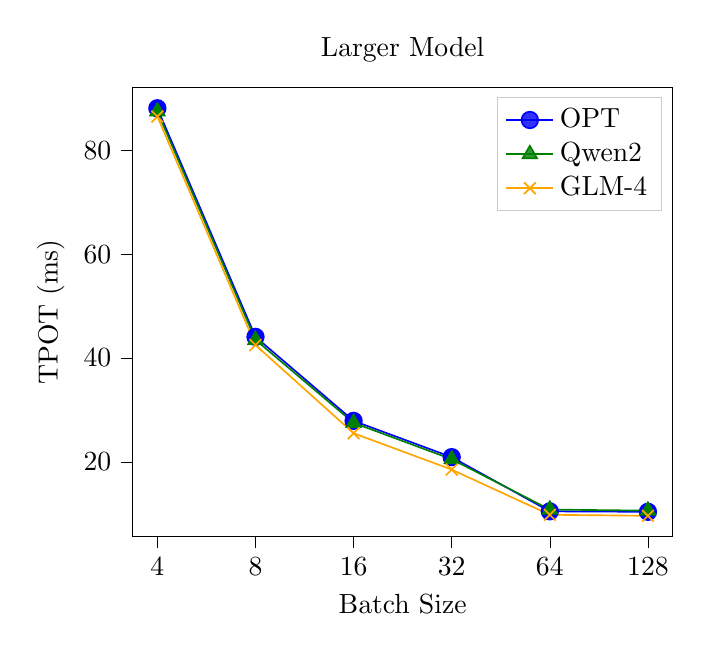
\begin{tikzpicture}

\definecolor{darkgray176}{RGB}{176,176,176}
\definecolor{green}{RGB}{0,128,0}
\definecolor{lightgray204}{RGB}{204,204,204}
\definecolor{orange}{RGB}{255,165,0}

\begin{axis}[
legend cell align={left},
legend style={fill opacity=0.8, draw opacity=1, text opacity=1, draw=lightgray204},
tick align=outside,
tick pos=left,
title={Larger Model},
x grid style={darkgray176},
xlabel={Batch Size},
xmin=-0.25, xmax=5.25,
xtick style={color=black},
xtick={0,1,2,3,4,5},
xtick={0,1,2,3,4,5},
xtick={0,1,2,3,4,5},
xtick={0,1,2,3,4,5},
xticklabels={4,8,16,32,64,128},
xticklabels={4,8,16,32,64,128},
xticklabels={4,8,16,32,64,128},
xticklabels={4,8,16,32,64,128},
y grid style={darkgray176},
ylabel={TPOT (ms)},
ymin=5.675, ymax=92.025,
ytick style={color=black}
]
\addplot [semithick, blue, mark=*, mark size=3, mark options={solid}]
table {%
0 88.1
1 44.066
2 27.8875
3 20.9
4 10.46
5 10.37
};
\addlegendentry{OPT}
\addplot [semithick, green, mark=triangle*, mark size=3, mark options={solid}]
table {%
0 87.5
1 43.5
2 27.5
3 20.5
4 10.8
5 10.6
};
\addlegendentry{Qwen2}
\addplot [semithick, orange, mark=x, mark size=3, mark options={solid}]
table {%
0 86.5
1 42.5
2 25.5
3 18.5
4 9.8
5 9.6
};
\addlegendentry{GLM-4}
\end{axis}

\end{tikzpicture}
 % 插入 TikZ 图
 }
    \caption{TPOT of different models using \sys.}
    \label{fig:eval3}
\end{figure}

\PN{Supporting more input and output tokens.}
In our experiments, we use the Qwen2-7B model, which support a maximum position embedding size of 32,768 tokens. 
This choice is deliberate, 
as this model significantly exceed the position embedding limits of OPT models and Yi-1.5 model, 
ensuring that the system remains capable of processing long input sequences. 
To compare with \flexgen, we calculate the corresponding offloading ratio based on the \interval values used in \sys and then manually set this ratio in \flexgen. 
We also conducted comparisons with \deepspeed.

The results in Figure~\ref{fig:eval4} show that, 
\sys supports larger max length than others. 
This is because reducing the GPU memory using allows \sys to allocate more GPU memory for token processing, thereby increasing the maximum allocatable length. 
As a result, the system can support larger batch sizes, 
longer input sequences, or extended output sequences under different interval settings, which helps to improve throughput. 
In contrast, \flexgen consistently shows smaller max length than \sys, while \deepspeed always retains one layer in GPU HBM, 
resulting in a constant larger value in the graph.

\begin{figure}[t]
    \centering
    \resizebox{\columnwidth}{!}{
        % This file was created with tikzplotlib v0.10.1.
\begin{tikzpicture}

\definecolor{darkgray176}{RGB}{176,176,176}
\definecolor{darkorange25512714}{RGB}{255,127,14}
\definecolor{forestgreen4416044}{RGB}{44,160,44}
\definecolor{lightgray204}{RGB}{204,204,204}
\definecolor{steelblue31119180}{RGB}{31,119,180}

\begin{groupplot}[group style={group size=2 by 1}]
\nextgroupplot[
legend cell align={left},
legend style={
  fill opacity=0.8,
  draw opacity=1,
  text opacity=1,
  at={(0.91,0.5)},
  anchor=east,
  draw=lightgray204
},
tick align=outside,
tick pos=left,
title={Qwen2 Model},
x grid style={darkgray176},
xlabel={Interval},
xmajorgrids,
xmin=1.7, xmax=8.3,
xtick style={color=black},
y grid style={darkgray176},
ylabel={Max Length},
ymajorgrids,
ymin=7835.44, ymax=25817.36,
ytick style={color=black}
]
\addplot [semithick, steelblue31119180, mark=*, mark size=3, mark options={solid}]
table {%
2 20080
3 15440
4 13904
5 12352
6 11584
7 10816
8 10816
};
\addlegendentry{Original}
\addplot [semithick, darkorange25512714, mark=triangle*, mark size=3, mark options={solid}]
table {%
2 16064
3 12352
4 11123.2
5 9881.6
6 9267.2
7 8652.8
8 8652.8
};
\addlegendentry{FlexGen}
\addplot [semithick, forestgreen4416044, dashed]
table {%
1.7 25000
8.3 25000
};
\addlegendentry{DeepSpeed}
\addplot [semithick, red, dashed]
table {%
1.7 9376
8.3 9376
};
\addlegendentry{Naive}

\nextgroupplot[
legend cell align={left},
legend style={
  fill opacity=0.8,
  draw opacity=1,
  text opacity=1,
  at={(0.91,0.5)},
  anchor=east,
  draw=lightgray204
},
tick align=outside,
tick pos=left,
title={GLM-4 Model},
x grid style={darkgray176},
xlabel={Interval},
xmajorgrids,
xmin=1.7, xmax=8.3,
xtick style={color=black},
y grid style={darkgray176},
ylabel={Max Length},
ymajorgrids,
ymin=7835.44, ymax=25817.36,
ytick style={color=black}
]
\addplot [semithick, steelblue31119180, mark=*, mark size=3, mark options={solid}]
table {%
2 20080
3 15440
4 13904
5 12352
6 11584
7 10816
8 10816
};
\addlegendentry{Original}
\addplot [semithick, darkorange25512714, mark=triangle*, mark size=3, mark options={solid}]
table {%
2 16064
3 12352
4 11123.2
5 9881.6
6 9267.2
7 8652.8
8 8652.8
};
\addlegendentry{FlexGen}
\addplot [semithick, forestgreen4416044, dashed]
table {%
1.7 25000
8.3 25000
};
\addlegendentry{DeepSpeed}
\addplot [semithick, red, dashed]
table {%
1.7 9376
8.3 9376
};
\addlegendentry{Naive}
\end{groupplot}

\end{tikzpicture}
 % 插入 TikZ 图
 }
    \caption{Maximum prompt length the model can process under different \interval settings.
 The dashed line represents the maximum length in the naive mode.}
    \label{fig:eval4}
\end{figure}



\subsection{Profiling Accuracy}

This subsection evaluates the effectiveness of the \interval analyzer, namely examining the optimality of the \interval value determined during the record-generating phase. 
\Maphsge{batch size to 128. }
Based on the optimal \interval value from the records, we conducted experiments under both the optimal and alternative \interval configurations, 
evaluating TPOT latency and recording the corresponding GPU memory usage for each setting.

The results are shown in Figure~\ref{fig:profileraccu}. 
According to performance records, the optimal \interval values are identified as 3 for the Qwen2 and GLM-4 models and 4 for the OPT and LLaMA model. 
The optimal \interval values achieve an effective balance by ensuring compliance with TPOT SLO while minimizing GPU memory usage. 
When \interval is smaller than the optimal value, GPU memory usage is reduced; 
however, this comes at the cost of SLO violations due to increased latency resulting in degraded throughput. 

\Maphsge{shown in fig, larger...}
In contrast, larger \interval values consistently satisfy the SLO but incur significant memory overhead without measurable performance gains. 
Specially, when the model size exceeds the available GPU memory, there is a practical upper bound on the \interval setting. 
As illustrated in the results for the OPT-13B model, which has a size of 26GB, this exceeds the 24GB GPU memory of the A10 GPU. 
Consequently, when the \interval value surpasses 5, the model cannot be deployed due to out-of-memory (OOM) errors.

\begin{figure}[t]
    \centering
    \resizebox{\columnwidth}{!}{
        % This file was created with tikzplotlib v0.10.1.
\begin{tikzpicture}

\definecolor{crimson2143940}{RGB}{214,39,40}
\definecolor{darkgray176}{RGB}{176,176,176}
\definecolor{forestgreen4416044}{RGB}{44,160,44}
\definecolor{lightgray204}{RGB}{204,204,204}
\definecolor{steelblue31119180}{RGB}{31,119,180}

\begin{groupplot}[group style={group size=2 by 1}]
\nextgroupplot[
legend cell align={left},
legend style={fill opacity=0.8, draw opacity=1, text opacity=1, draw=lightgray204},
tick align=outside,
tick pos=left,
title={(a) TPOT Analysis},
x grid style={darkgray176},
xlabel={Interval Configuration},
xmin=-0.56125, xmax=4.08625,
xtick style={color=black},
xtick={0,1.175,2.35,3.525},
xticklabels={5,6,8,10},
y grid style={darkgray176},
ylabel={TPOT},
ymin=0, ymax=130.1265,
ytick style={color=black}
]
\draw[draw=none,fill=steelblue31119180] (axis cs:-0.35,0) rectangle (axis cs:0,123.93);
\addlegendimage{ybar,ybar legend,draw=none,fill=steelblue31119180}
\addlegendentry{OPT}

\draw[draw=none,fill=steelblue31119180] (axis cs:0.825,0) rectangle (axis cs:1.175,115.03);
\draw[draw=none,fill=steelblue31119180] (axis cs:2,0) rectangle (axis cs:2.35,89.388);
\draw[draw=none,fill=steelblue31119180] (axis cs:3.175,0) rectangle (axis cs:3.525,68.17);
\draw[draw=forestgreen4416044,fill=white,postaction={pattern=north east lines, pattern color=forestgreen4416044}] (axis cs:2.77555756156289e-17,0) rectangle (axis cs:0.35,123.93);
\addlegendimage{ybar,ybar legend,draw=forestgreen4416044,fill=white,postaction={pattern=north east lines, pattern color=forestgreen4416044}}
\addlegendentry{Qwen2}

\draw[draw=forestgreen4416044,fill=white,postaction={pattern=north east lines, pattern color=forestgreen4416044}] (axis cs:1.175,0) rectangle (axis cs:1.525,115.03);
\draw[draw=forestgreen4416044,fill=white,postaction={pattern=north east lines, pattern color=forestgreen4416044}] (axis cs:2.35,0) rectangle (axis cs:2.7,89.388);
\draw[draw=forestgreen4416044,fill=white,postaction={pattern=north east lines, pattern color=forestgreen4416044}] (axis cs:3.525,0) rectangle (axis cs:3.875,68.17);
\addplot [semithick, crimson2143940, dashed]
table {%
-0.56125 90
4.08625 90
};
\addlegendentry{SLO}

\nextgroupplot[
legend cell align={left},
legend style={
  fill opacity=0.8,
  draw opacity=1,
  text opacity=1,
  at={(0.03,0.97)},
  anchor=north west,
  draw=lightgray204
},
tick align=outside,
tick pos=left,
title={(b) Memory Usage Analysis},
x grid style={darkgray176},
xlabel={Configuration},
xmin=-0.7375, xmax=7.7875,
xtick style={color=black},
xtick={0,1.175,2.35,3.525,4.7,5.875,7.05},
xticklabels={2,3,4,5,6,8,10},
y grid style={darkgray176},
ylabel={Memory Usage (GB)},
ymin=0, ymax=22.96875,
ytick style={color=black}
]
\draw[draw=none,fill=steelblue31119180] (axis cs:-0.35,0) rectangle (axis cs:0,11.5);
\draw[draw=none,fill=steelblue31119180] (axis cs:0.825,0) rectangle (axis cs:1.175,15.8);
\draw[draw=none,fill=steelblue31119180] (axis cs:2,0) rectangle (axis cs:2.35,17.25);
\draw[draw=none,fill=steelblue31119180] (axis cs:3.175,0) rectangle (axis cs:3.525,18.69);
\draw[draw=none,fill=steelblue31119180] (axis cs:4.35,0) rectangle (axis cs:4.7,21.125);
\draw[draw=none,fill=steelblue31119180] (axis cs:5.525,0) rectangle (axis cs:5.875,21.5);
\draw[draw=none,fill=steelblue31119180] (axis cs:6.7,0) rectangle (axis cs:7.05,21.875);
\draw[draw=forestgreen4416044,fill=white,postaction={pattern=north east lines, pattern color=forestgreen4416044}] (axis cs:2.77555756156289e-17,0) rectangle (axis cs:0.35,11.5);
\draw[draw=forestgreen4416044,fill=white,postaction={pattern=north east lines, pattern color=forestgreen4416044}] (axis cs:1.175,0) rectangle (axis cs:1.525,15.8);
\draw[draw=forestgreen4416044,fill=white,postaction={pattern=north east lines, pattern color=forestgreen4416044}] (axis cs:2.35,0) rectangle (axis cs:2.7,17.25);
\draw[draw=forestgreen4416044,fill=white,postaction={pattern=north east lines, pattern color=forestgreen4416044}] (axis cs:3.525,0) rectangle (axis cs:3.875,18.69);
\draw[draw=forestgreen4416044,fill=white,postaction={pattern=north east lines, pattern color=forestgreen4416044}] (axis cs:4.7,0) rectangle (axis cs:5.05,21.125);
\draw[draw=forestgreen4416044,fill=white,postaction={pattern=north east lines, pattern color=forestgreen4416044}] (axis cs:5.875,0) rectangle (axis cs:6.225,21.5);
\draw[draw=forestgreen4416044,fill=white,postaction={pattern=north east lines, pattern color=forestgreen4416044}] (axis cs:7.05,0) rectangle (axis cs:7.4,21.875);
\end{groupplot}

\end{tikzpicture}
 % 插入 TikZ 图
 }
    \caption{The TTFT, TPOT, and memory usage of \sys under different \interval configurations. 
 The red dashed lines represent the SLO. The optimal \interval is 3 in (a) and 8 in (b).}
    \label{fig:profileraccu}
\end{figure}

\DZ{Missing breakdown analysis.}
\subsection{Latency Breakdown}
\Maphsge{Add a figure here.}

To understand \sys's performance in detail, we conduct a latency breakdown analysis of its execution process. 
Specifically, we divide the lifecycle of a single iteration in \sys into the following stages: inference execution, transfer blocking, and \interval adjustment. 
For each stage, we accumulate the total time consumed across all requests to determine its proportion in the overall system execution time. 
We compare \sys with other baseline systems, selecting the OPT-13B model for evaluation since it is natively supported by \flexgen. 

The results of the latency breakdown are illustrated in Figure~X. 
As shown, the primary performance bottleneck in \deepspeed lies in data transfer overhead, which accounts for X\% of the total execution time—significantly 
higher than that in \sys. Although \flexgen exhibits slightly lower data transfer overhead compared to \sys, 
this is largely attributed to its insufficient utilization of host memory resources. 
On the other hand, the overhead introduced by \interval adjustment in \sys is minimal, occupying only a negligible portion of the iteration lifecycle. 

\subsection{Bandwidth contention}

We conduct experiments simulating a scenario where two GPUs share PCIe bandwidth. In this setup, we run inference tasks on both GPUs simultaneously, 
measuring SLO and throughput. Specifically, we run the OPT model on FlexGen, while conducting experiments with different models on \sys. 

Figure~\ref{fig:evalband}(a) shows the SLO results, where \sys consistently maintains the SLO, while FlexGen fails to do so. 
This is because FlexGen lacks the ability to dynamically adjust the offload ratio, whereas \sys can adaptively adjust the \interval to reduce data transfers. 
As a result, FlexGen exhibits lower throughput compared to \sys, as shown in Figure~\ref{fig:evalband}(b).


\begin{figure}[t]
    \centering
    \resizebox{0.9\columnwidth}{!}{
        % This file was created with tikzplotlib v0.10.1.
\begin{tikzpicture}

\definecolor{chocolate213940}{RGB}{213,94,0}
\definecolor{darkgray176}{RGB}{176,176,176}
\definecolor{darkgreen}{RGB}{0,100,0}
\definecolor{darkorange}{RGB}{255,140,0}
\definecolor{gray}{RGB}{128,128,128}

\begin{axis}[
height=6cm,
legend cell align={left},
legend columns=3,
legend style={fill opacity=0.8, draw opacity=1, text opacity=1, at={(0.5,1.2)}, anchor=north, draw=none},
tick align=outside,
tick pos=left,
width=14cm,
x grid style={darkgray176},
xlabel={Batch Size},
xmin=-0.662, xmax=4.662,
xtick style={color=black},
xtick={0,1,2,3,4},
xticklabels={4,8,16,32,64},
y grid style={darkgray176},
ylabel={TPOT (ms)},
ymin=0, ymax=166.95,
ytick style={color=black}
]
\draw[draw=none,fill=chocolate213940] (axis cs:-0.42,0) rectangle (axis cs:-0.14,154);
\addlegendimage{ybar,ybar legend,draw=none,fill=chocolate213940}
\addlegendentry{NovaServe-OPT}

\draw[draw=none,fill=chocolate213940] (axis cs:0.58,0) rectangle (axis cs:0.86,76.99);
\draw[draw=none,fill=chocolate213940] (axis cs:1.58,0) rectangle (axis cs:1.86,39.91);
\draw[draw=none,fill=chocolate213940] (axis cs:2.58,0) rectangle (axis cs:2.86,20.16);
\draw[draw=none,fill=chocolate213940] (axis cs:3.58,0) rectangle (axis cs:3.86,10.08);
\draw[draw=darkorange,fill=white,semithick,postaction={pattern=grid, pattern color=darkorange}] (axis cs:-0.14,0) rectangle (axis cs:0.14,159);
\addlegendimage{ybar,ybar legend,draw=darkorange,fill=white,semithick,postaction={pattern=grid, pattern color=darkorange}}
\addlegendentry{NovaServe-Qwen}

\draw[draw=darkorange,fill=white,semithick,postaction={pattern=grid, pattern color=darkorange}] (axis cs:0.86,0) rectangle (axis cs:1.14,81.756375);
\draw[draw=darkorange,fill=white,semithick,postaction={pattern=grid, pattern color=darkorange}] (axis cs:1.86,0) rectangle (axis cs:2.14,40.63);
\draw[draw=darkorange,fill=white,semithick,postaction={pattern=grid, pattern color=darkorange}] (axis cs:2.86,0) rectangle (axis cs:3.14,20.31803125);
\draw[draw=darkorange,fill=white,semithick,postaction={pattern=grid, pattern color=darkorange}] (axis cs:3.86,0) rectangle (axis cs:4.14,10.159015625);
\draw[draw=darkgreen,fill=white,semithick,postaction={pattern=vertical lines, pattern color=darkgreen}] (axis cs:0.14,0) rectangle (axis cs:0.42,0);
\addlegendimage{ybar,ybar legend,draw=darkgreen,fill=white,semithick,postaction={pattern=vertical lines, pattern color=darkgreen}}
\addlegendentry{FlexGen-OPT}

\draw[draw=darkgreen,fill=white,semithick,postaction={pattern=vertical lines, pattern color=darkgreen}] (axis cs:1.14,0) rectangle (axis cs:1.42,114.75);
\draw[draw=darkgreen,fill=white,semithick,postaction={pattern=vertical lines, pattern color=darkgreen}] (axis cs:2.14,0) rectangle (axis cs:2.42,100.43);
\draw[draw=darkgreen,fill=white,semithick,postaction={pattern=vertical lines, pattern color=darkgreen}] (axis cs:3.14,0) rectangle (axis cs:3.42,58.44);
\draw[draw=darkgreen,fill=white,semithick,postaction={pattern=vertical lines, pattern color=darkgreen}] (axis cs:4.14,0) rectangle (axis cs:4.42,29.22);
\addplot [gray, dashed, forget plot]
table {%
-0.662 100
4.662 100
};
\end{axis}

\end{tikzpicture}
 % 插入 TikZ 图
 }
    \caption{TPOT comparison of \sys (OPT-13B and LLaMA-13B models) and FlexGen (OPT-13B model) under contention environments across different batch sizes.
 The dashed line represents the SLO.}
    \label{fig:evalband}
\end{figure}





% %-------------------------------------------------------------------------------
\section{Related Work}
%-------------------------------------------------------------------------------
\label{sec:relwk}

\DZ{Most text in this section can be removed.}

\PN{Efficient LLM serving.} 
Several recent studies address these challenges by proposing methods to enhance system performance and resource efficiency in LLM inference. 
Orca\cite{orca} introduces continuous batching to enhance GPU throughput. 
vLLM\cite{vllm} leverages PageAttention to optimize Key-Value~(KV) cache memory usage, enabling efficient resource allocation. 
SARATHI\cite{sarathi} adopts a chunked-prefill strategy, dividing prefill requests into smaller chunks while combining them with decoding requests to achieve better hardware utilization. 
StreamingLLM\cite{StreamingLLM} extends LLM capabilities by allowing the generation of sequence lengths beyond their original training limits. 
\sys builds on some of these techniques like vLLM, and is designed to work in parallel with other approaches to further enhance performance and resource efficiency.

\PN{Offloading techniques.}
Existing works have explored various techniques to improve large-scale model inference performance, particularly on resource-constrained hardware. 
Systems such as DeepSpeed ZeRO-Inference\cite{zero-infer} and Hugging Face Accelerate\cite{huggingface} adopt offloading strategies originally designed for training scenarios. 
Infinite-LLM\cite{lin2024infinitellmefficientllmservice} manages the utilization of all GPU and CPU memory resources to store the KV cache.
These approaches may still cause computation to stall as they do not ensure data readiness at the required time.
InfiniGen\cite{infinigen} mitigates KV cache fetch overhead by speculatively prefetching essential KV entries, improving cache management efficiency. 
\textsc{Neo}\cite{jiangxuanlin} offloads part of attention compute and KV cache states from GPU to CPU to balance compute and memory resources.
\textsc{Aqua}~\cite{aqua} proposes a memory disaggregation mechanism that decouples memory from compute, enabling GPUs to share surplus memory across the system.
These three works cannot handle models that exceed the GPU memory capacity, making them orthogonal to our approach.

% \PN{Scheduling systems.} 
% Recent works have explored efficient resource scheduling and allocation strategies for deep learning tasks, focusing on optimizing throughput\cite{pollux}, 
% heterogeneous-aware scheduling\cite{sia}, preemption and latency-aware scheduling\cite{Clockwork, SHEPHERD}, 
% and improving resource utilization through model parallelism\cite{AlpaServe} or iteration-level preemptive scheduling to mitigate queueing delays\cite{fastserve}.
% There are also concurrent works that employ disaggregation techniques to decouple and balance resource allocation, 
% improving efficiency in LLM inference, such as Splitwise\cite{splitwise}, TetriInfer\cite{TetriInfer}, DéjàVu\cite{dejavu}, and Distserve\cite{distserve}
% \sys is orthogonal to the large body of work on scheduling, as its separation of prefill and decoding stages can be implemented using any of the aforementioned approaches.



% %-------------------------------------------------------------------------------
\section{Conclusion}
%-------------------------------------------------------------------------------

This paper presents \sys, a memory offloading mechanism
for LLM serving that meets latency SLOs while maximizing the host 
memory usage. 
%
\sys captures the tradeoff between meeting SLOs and maximizing host memory usage 
with \interval, an internal tunable knob. 
%
In addition, \sys automatically decides the optimal \interval, \ie, the smallest \interval that meets SLOs, with a two-stage tuning approach.  
%
The first stage assumes bandwidth contention and profiles the GPU model offline, and generates a performance \record that, for any valid combination of SLOs, sequence lengths, and batching sizes, stores an optimal \interval,
%
The second stage adjusts the \interval for GPU instances sharing the bus to ensure that the SLOs can still be met while maximizing the aggregate host memory usage across all GPU instances. 
%
Our evaluation shows that \sys consistently maintains SLO under various runtime
scenarios, and outperforms \flexgen in throughput by 1.85\X, due to use 2.37\X more host memory. 



\begin{thebibliography}{00}
\bibitem{b1} G. Eason, B. Noble, and I. N. Sneddon, ``On certain integrals of Lipschitz-Hankel type involving products of Bessel functions,'' Phil. Trans. Roy. Soc. London, vol. A247, pp. 529--551, April 1955.
\bibitem{b2} J. Clerk Maxwell, A Treatise on Electricity and Magnetism, 3rd ed., vol. 2. Oxford: Clarendon, 1892, pp.68--73.
\bibitem{b3} I. S. Jacobs and C. P. Bean, ``Fine particles, thin films and exchange anisotropy,'' in Magnetism, vol. III, G. T. Rado and H. Suhl, Eds. New York: Academic, 1963, pp. 271--350.
\bibitem{b4} K. Elissa, ``Title of paper if known,'' unpublished.
\bibitem{b5} R. Nicole, ``Title of paper with only first word capitalized,'' J. Name Stand. Abbrev., in press.
\bibitem{b6} Y. Yorozu, M. Hirano, K. Oka, and Y. Tagawa, ``Electron spectroscopy studies on magneto-optical media and plastic substrate interface,'' IEEE Transl. J. Magn. Japan, vol. 2, pp. 740--741, August 1987 [Digests 9th Annual Conf. Magnetics Japan, p. 301, 1982].
\bibitem{b7} M. Young, The Technical Writer's Handbook. Mill Valley, CA: University Science, 1989.
\bibitem{b8} D. P. Kingma and M. Welling, ``Auto-encoding variational Bayes,'' 2013, arXiv:1312.6114. [Online]. Available: https://arxiv.org/abs/1312.6114
\bibitem{b9} S. Liu, ``Wi-Fi Energy Detection Testbed (12MTC),'' 2023, gitHub repository. [Online]. Available: https://github.com/liustone99/Wi-Fi-Energy-Detection-Testbed-12MTC
\bibitem{b10} ``Treatment episode data set: discharges (TEDS-D): concatenated, 2006 to 2009.'' U.S. Department of Health and Human Services, Substance Abuse and Mental Health Services Administration, Office of Applied Studies, August, 2013, DOI:10.3886/ICPSR30122.v2
\bibitem{b11} K. Eves and J. Valasek, ``Adaptive control for singularly perturbed systems examples,'' Code Ocean, Aug. 2023. [Online]. Available: https://codeocean.com/capsule/4989235/tree
\end{thebibliography}

\vspace{12pt}
\color{red}
IEEE conference templates contain guidance text for composing and formatting conference papers. Please ensure that all template text is removed from your conference paper prior to submission to the conference. Failure to remove the template text from your paper may result in your paper not being published.

\end{document}
